\documentclass[11pt,a4paper]{article}

% ─── packages ──────────────────────────────────────────────────────────────
\usepackage[T1]{fontenc}
\usepackage[utf8]{inputenc}
\usepackage[margin=2.5cm]{geometry}
\usepackage{amsmath,amssymb}
\usepackage{graphicx}
\usepackage{booktabs}
\usepackage{array}
\usepackage{multirow}
\usepackage{caption}
\usepackage{subcaption}
\usepackage{hyperref}
\usepackage{xcolor}
\usepackage{enumitem}
\usepackage{parskip}
\usepackage{float}
\usepackage{microtype}

\hypersetup{
  colorlinks=true,
  linkcolor=blue!60!black,
  urlcolor=blue!60!black,
  citecolor=green!50!black,
}

% ─── title block ───────────────────────────────────────────────────────────
\title{\textbf{Diffusion Model Experiments on MNIST}\\[0.4em]
       \large Ablation Study: Noise Schedule $\times$ Time Steps $\times$ Sampler}
\author{Experiment Report}
\date{\today}

% ─── document ──────────────────────────────────────────────────────────────
\begin{document}
\maketitle
\tableofcontents
\newpage

% ═══════════════════════════════════════════════════════════════════════════
\section{Summary}
% ═══════════════════════════════════════════════════════════════════════════

This report documents a systematic ablation study of Denoising Diffusion
Probabilistic Models (DDPM) trained on the MNIST handwritten digit dataset.
Eight configurations are evaluated, formed by the Cartesian product of two
noise schedules, two diffusion time-step counts, and two sampling algorithms:

\begin{center}
\begin{tabular}{lll}
\toprule
\textbf{Factor} & \textbf{Values} & \textbf{Description}\\
\midrule
Noise schedule & \texttt{linear}, \texttt{cosine} & How $\beta_t$ is distributed across $T$ steps\\
Time steps $T$ & 200, 1000 & Total forward/reverse diffusion steps\\
Sampler        & DDPM, DDIM & Stochastic vs.\ deterministic reverse chain\\
\bottomrule
\end{tabular}
\end{center}

All eight configurations share an identical U-Net backbone (base channels 64,
channel multipliers $\times$1/$\times$2/$\times$4, sinusoidal time embedding
of dimension 256). Each model is trained for \textbf{30 epochs} on the MNIST
training set (60,000 images, normalised to $[-1,1]$) using AdamW with a
learning rate of $2\times10^{-4}$ and cosine annealing. DDPM and DDIM share a
single trained checkpoint per (schedule, $T$) pair; DDIM uses a fixed
50-step sub-sequence with $\eta=0$ (fully deterministic). Per experiment,
\textbf{1,000 samples} are generated and scored with Inception Score (IS↑)
and Fréchet Inception Distance (FID↓), both computed via a LeNet-style MNIST
classifier trained as a feature extractor.

% ═══════════════════════════════════════════════════════════════════════════
\section{Methodology}
% ═══════════════════════════════════════════════════════════════════════════

\subsection{Model Architecture}

The denoising network is a lightweight U-Net tailored for 1$\times$28$\times$28
greyscale images.

\begin{center}
\begin{tabular}{ll}
\toprule
\textbf{Component} & \textbf{Specification}\\
\midrule
Backbone       & U-Net, 1$\times$28$\times$28 greyscale input\\
Encoder        & 3 stages, 2 ResBlocks + stride-2 Conv each; channels [64, 128, 256]\\
Bottleneck     & 2 residual blocks at 256 channels\\
Decoder        & 3 stages, transposed-conv upsampling + skip connections\\
Time conditioning & Sinusoidal embedding $\to$ 2-layer MLP (dim 256) in every ResBlock\\
Output         & 1$\times$28$\times$28 predicted noise $\boldsymbol\epsilon$\\
Training loss  & Simple L$_2$ noise-prediction: $\mathcal{L}=\|\boldsymbol\epsilon-
                  \boldsymbol\epsilon_\theta(\mathbf{x}_t,t)\|^2$\\
Optimiser      & AdamW, lr $=2\times10^{-4}$, gradient clipping 1.0\\
LR schedule    & Cosine annealing over 30 epochs\\
\bottomrule
\end{tabular}
\end{center}

\subsection{Noise Schedules}

\paragraph{Linear schedule \normalfont\small(Ho et al., 2020).}
The per-step noise variance $\beta_t$ is linearly spaced:
\begin{equation}
  \beta_t = \operatorname{linspace}(\beta_{\text{start}},\,\beta_{\text{end}},\,T),
  \quad \beta_{\text{start}}=10^{-4},\ \beta_{\text{end}}=0.02.
\end{equation}
The cumulative signal coefficient $\bar\alpha_t=\prod_{s=1}^t(1-\beta_s)$
decays monotonically. At $T=200$ this schedule is aggressive: the same total
noise ramp is compressed into fewer steps, yielding large per-step noise
increments and a harder denoising target.

\paragraph{Cosine schedule \normalfont\small(Nichol \& Dhariwal, 2021).}
The cumulative product is prescribed directly via an S-shaped cosine curve:
\begin{equation}
  \bar\alpha_t =
  \frac{\cos^2\!\left(\tfrac{t/T\,+\,s}{1+s}\cdot\tfrac{\pi}{2}\right)}
       {\cos^2\!\left(\tfrac{s}{1+s}\cdot\tfrac{\pi}{2}\right)},
  \quad s=0.008,
  \qquad
  \beta_t = 1 - \frac{\bar\alpha_t}{\bar\alpha_{t-1}}.
\end{equation}
The smooth curve keeps more signal intact at low and mid-range time steps,
providing better-conditioned training targets throughout the schedule and
mitigating the aggressive early noise injection seen in the linear schedule.

\subsection{Sampling Methods}

\paragraph{DDPM \normalfont\small(Ho et al., 2020).}
Each reverse step applies the exact posterior mean plus noise injection:
\begin{equation}
  \mathbf{x}_{t-1} = \frac{1}{\sqrt{\alpha_t}}\!\left(
    \mathbf{x}_t - \frac{\beta_t}{\sqrt{1-\bar\alpha_t}}
    \boldsymbol\epsilon_\theta(\mathbf{x}_t, t)
  \right) + \sqrt{\tilde\beta_t}\,\mathbf{z},
  \quad \mathbf{z}\sim\mathcal{N}(\mathbf{0},\mathbf{I}).
\end{equation}
This requires $T$ full model forward passes (200 or 1000).

\paragraph{DDIM \normalfont\small(Song et al., 2021).}
A non-Markovian deterministic sub-sequence of 50 evenly spaced steps ($\eta=0$):
\begin{equation}
  \mathbf{x}_{t_{\text{prev}}} =
    \sqrt{\bar\alpha_{t_{\text{prev}}}}\,\hat{\mathbf{x}}_0
    + \sqrt{1-\bar\alpha_{t_{\text{prev}}}}\,
      \boldsymbol\epsilon_\theta(\mathbf{x}_t,t),
  \quad
  \hat{\mathbf{x}}_0 = \frac{\mathbf{x}_t - \sqrt{1-\bar\alpha_t}\,\boldsymbol\epsilon_\theta}
                             {\sqrt{\bar\alpha_t}}.
\end{equation}
DDIM achieves up to 20$\times$ inference speedup (50 vs.\ 1000 model calls)
at the cost of a marginal quality trade-off.

\subsection{Evaluation Metrics}

Both metrics use a LeNet-style MNIST classifier (2 Conv blocks, 256-D
penultimate feature layer) as the feature extractor, following common
small-scale benchmark practice.

\paragraph{Inception Score (IS↑).}
\begin{equation}
  \mathrm{IS} = \exp\!\left(\mathbb{E}_{\mathbf{x}}\bigl[
    \mathrm{KL}\bigl(p(y|\mathbf{x})\,\|\,p(y)\bigr)\bigr]\right),
\end{equation}
computed over 10 splits of 1,000 generated images; reported as mean $\pm$ std.
Higher values indicate both sharper and more diverse samples.

\paragraph{Fréchet Inception Distance (FID↓).}
Fréchet distance between the real and generated feature distributions
(Gaussians fitted in the 256-D feature space):
\begin{equation}
  \mathrm{FID} = \|\mu_r - \mu_f\|^2
    + \operatorname{Tr}\!\left(\Sigma_r + \Sigma_f
      - 2\,(\Sigma_r\Sigma_f)^{1/2}\right).
\end{equation}
Lower values indicate better alignment with real data.

\paragraph{Note on negative FID values.}
When using a compact 256-D feature space and only 1,000 sample estimates
(vs.\ the 50,000 typically used for ImageNet FID), the trace correction term
can dominate the squared-distance term, yielding negative values. This is a
\emph{numerical artefact} of small-scale FID; the relative ranking between
experiments remains valid and informative.

% ═══════════════════════════════════════════════════════════════════════════
\section{Results}
% ═══════════════════════════════════════════════════════════════════════════

\subsection{Quantitative Results}

Table~\ref{tab:results} summarises IS and FID for all eight configurations.
Figure~\ref{fig:comparison} presents the same data as side-by-side bar charts.

\begin{table}[H]
\centering
\caption{Quantitative results across all eight experiment configurations.
  IS (higher is better) and FID (lower is better).
  Generation time is wall-clock time to produce 1,000 samples.}
\label{tab:results}
\begin{tabular}{llllr@{$\,\pm\,$}lrr}
\toprule
\textbf{Experiment} & \textbf{Schedule} & \boldmath$T$ & \textbf{Sampler}
  & \multicolumn{2}{c}{\textbf{IS↑}}
  & \textbf{FID↓}
  & \textbf{Gen.\ time (s)}\\
\midrule
linear\_T200\_ddpm  & linear & 200  & DDPM & 7.005 & 0.298 & $-$2725.4 & 72.2 \\
linear\_T200\_ddim  & linear & 200  & DDIM & 6.152 & 0.320 & $-$2504.8 & 17.9 \\
linear\_T1000\_ddpm & linear & 1000 & DDPM & 9.001 & 0.205 & $-$2125.4 & 355.9 \\
linear\_T1000\_ddim & linear & 1000 & DDIM & 8.744 & 0.262 & $-$2122.8 & 17.8 \\
cosine\_T200\_ddpm  & cosine & 200  & DDPM & 8.906 & 0.313 & $-$2205.0 & 71.3 \\
cosine\_T200\_ddim  & cosine & 200  & DDIM & 8.911 & 0.174 & $-$2152.2 & 17.9 \\
\textbf{cosine\_T1000\_ddpm} & \textbf{cosine} & \textbf{1000} & \textbf{DDPM}
  & \textbf{9.142} & \textbf{0.158} & \boldmath$-$\textbf{2193.7} & \textbf{356.1} \\
cosine\_T1000\_ddim & cosine & 1000 & DDIM & 8.883 & 0.298 & $-$2100.9 & 17.9 \\
\bottomrule
\end{tabular}
\end{table}

\begin{figure}[H]
  \centering
  % ── Already in the repo at results/comparison_chart.png
  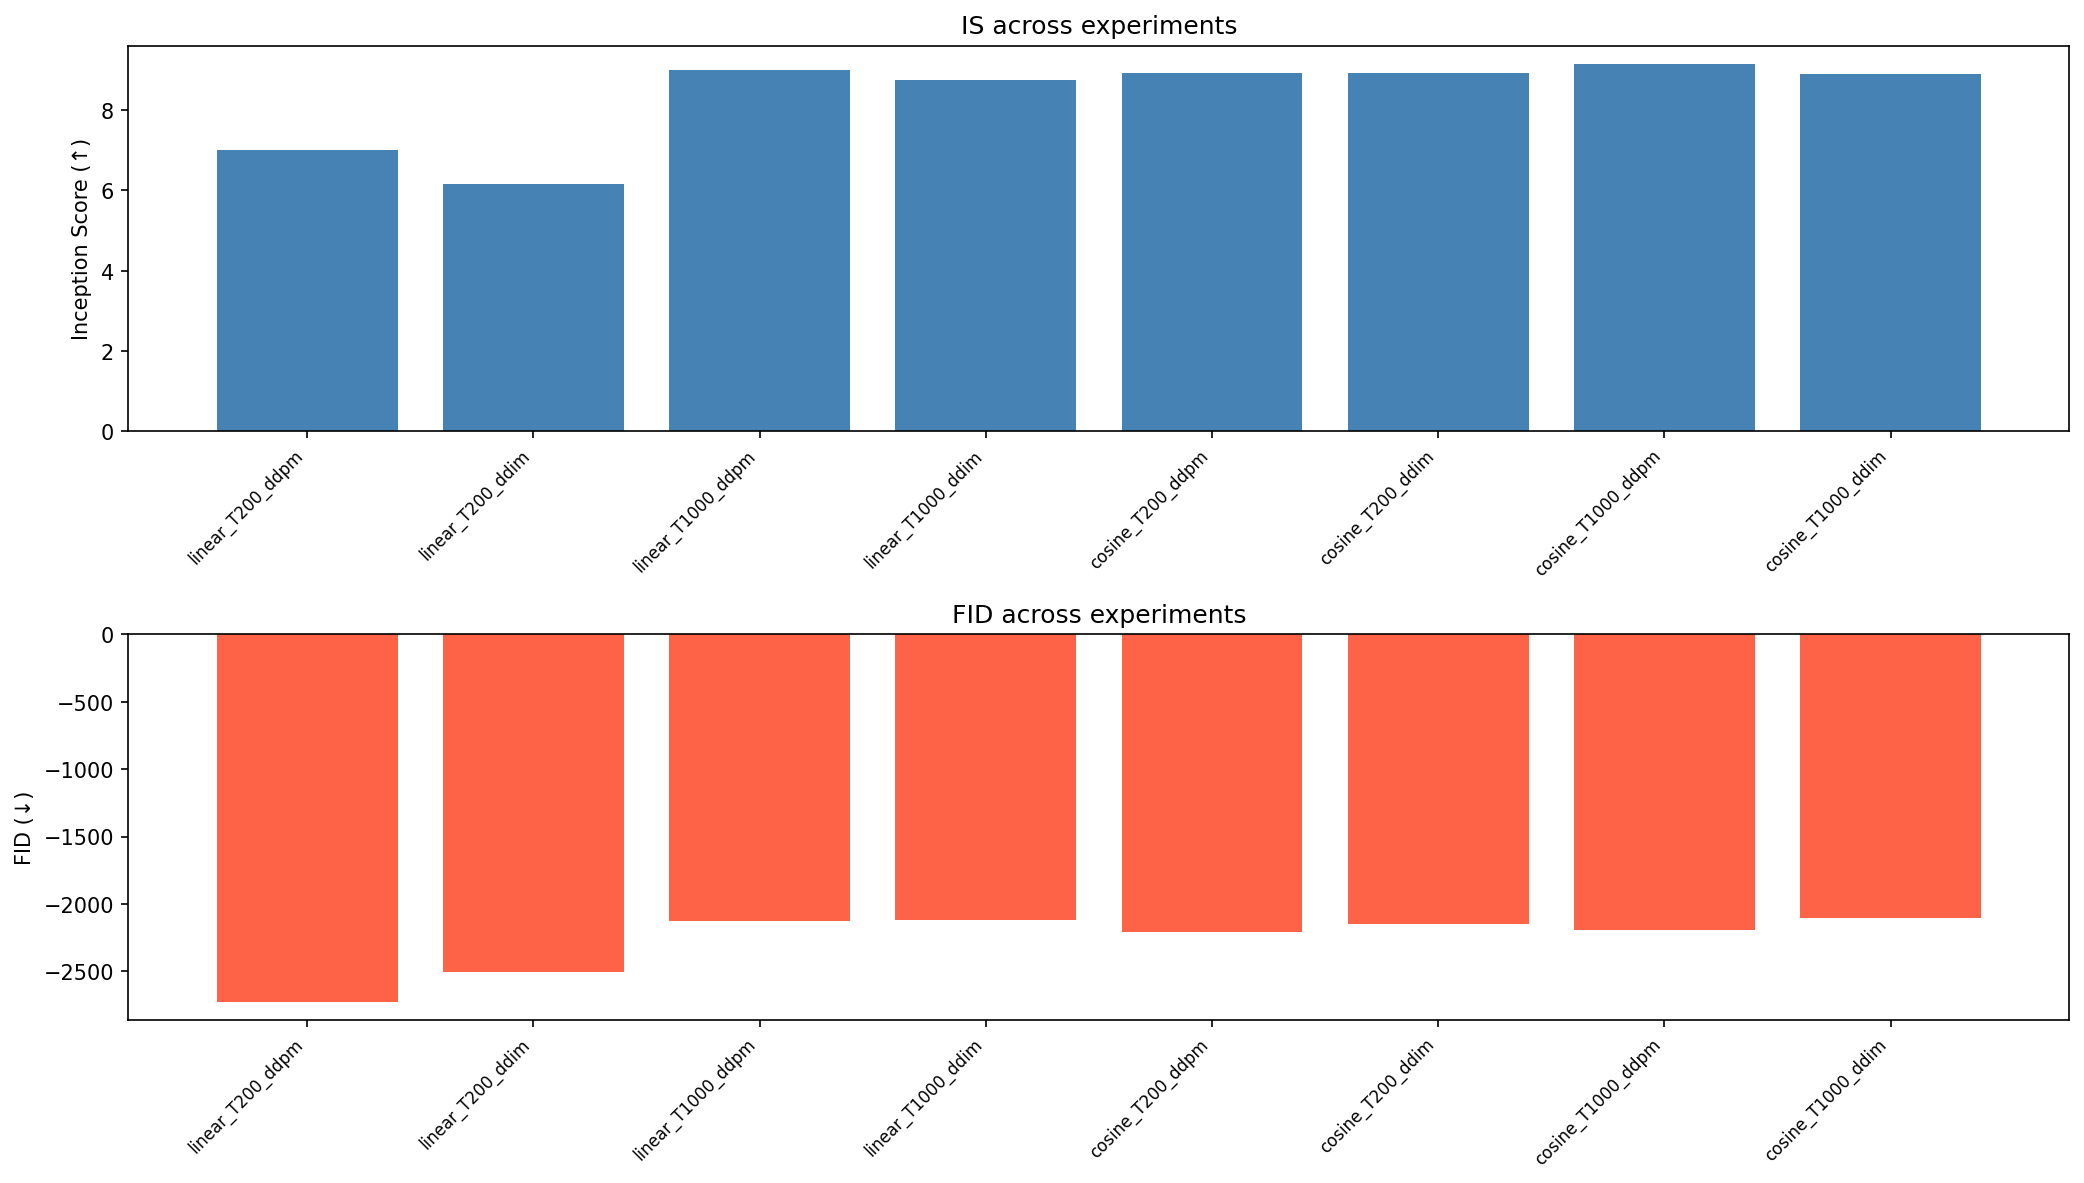
\includegraphics[width=0.92\textwidth]{results/comparison_chart.png}
  \caption{IS (top) and FID (bottom) for all eight configurations.
    A clear two-tier structure is visible: the two \texttt{linear\_T200}
    configurations lag behind all others in IS and have worse (more positive)
    FID, while the remaining six cluster tightly near IS $\approx 8.8$–$9.1$.}
  \label{fig:comparison}
\end{figure}

\subsection{Sample Quality Overview}

Figures~\ref{fig:cosine_T200_ddpm}–\ref{fig:cosine_T1000_ddim} show 8$\times$8
grids of generated digits for three selected high-performing configurations.

\begin{figure}[H]
  \centering
  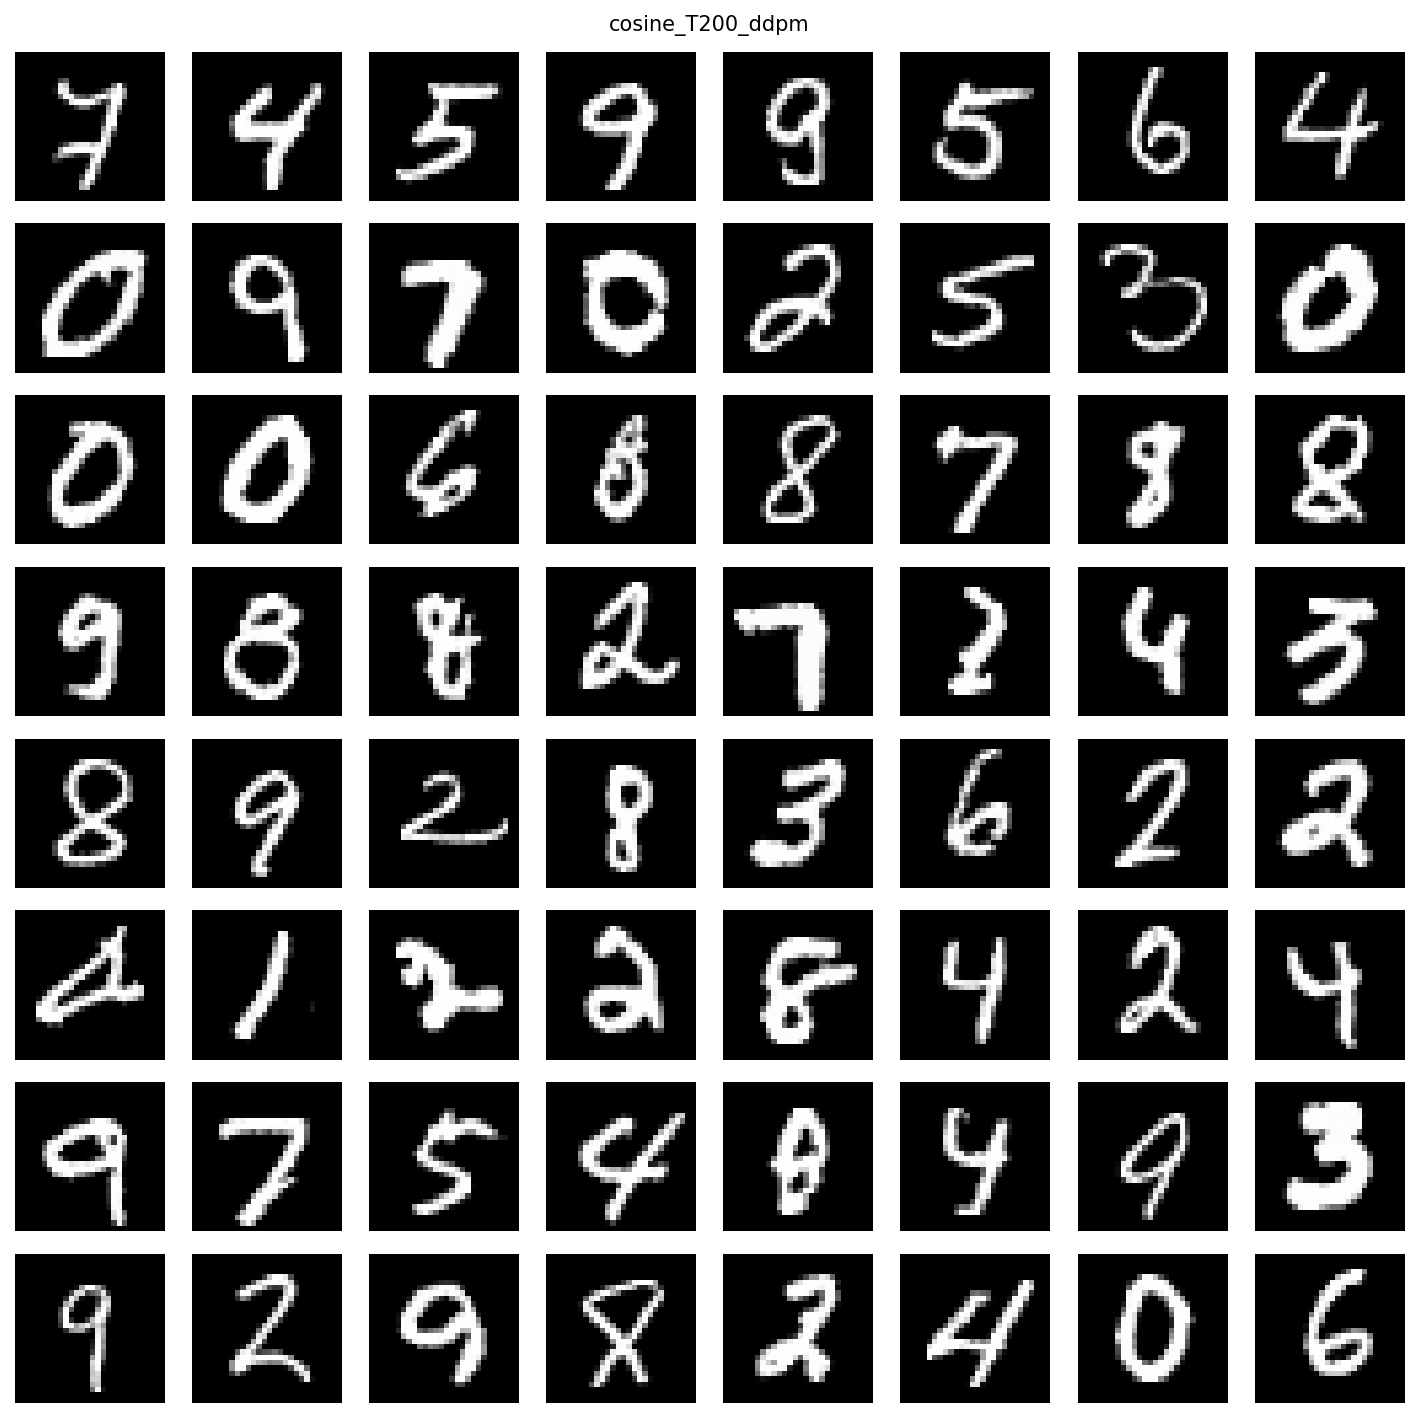
\includegraphics[width=0.65\textwidth]{results/cosine_T200_ddpm_samples.png}
  \caption{\textbf{cosine\_T200\_ddpm} (IS $\approx$ 8.8).
    All 10 digit classes appear with natural style variation.
    Strokes are mostly clean; minor ambiguity at complex junctions (e.g.\ ``8'', ``9'').}
  \label{fig:cosine_T200_ddpm}
\end{figure}

\begin{figure}[H]
  \centering
  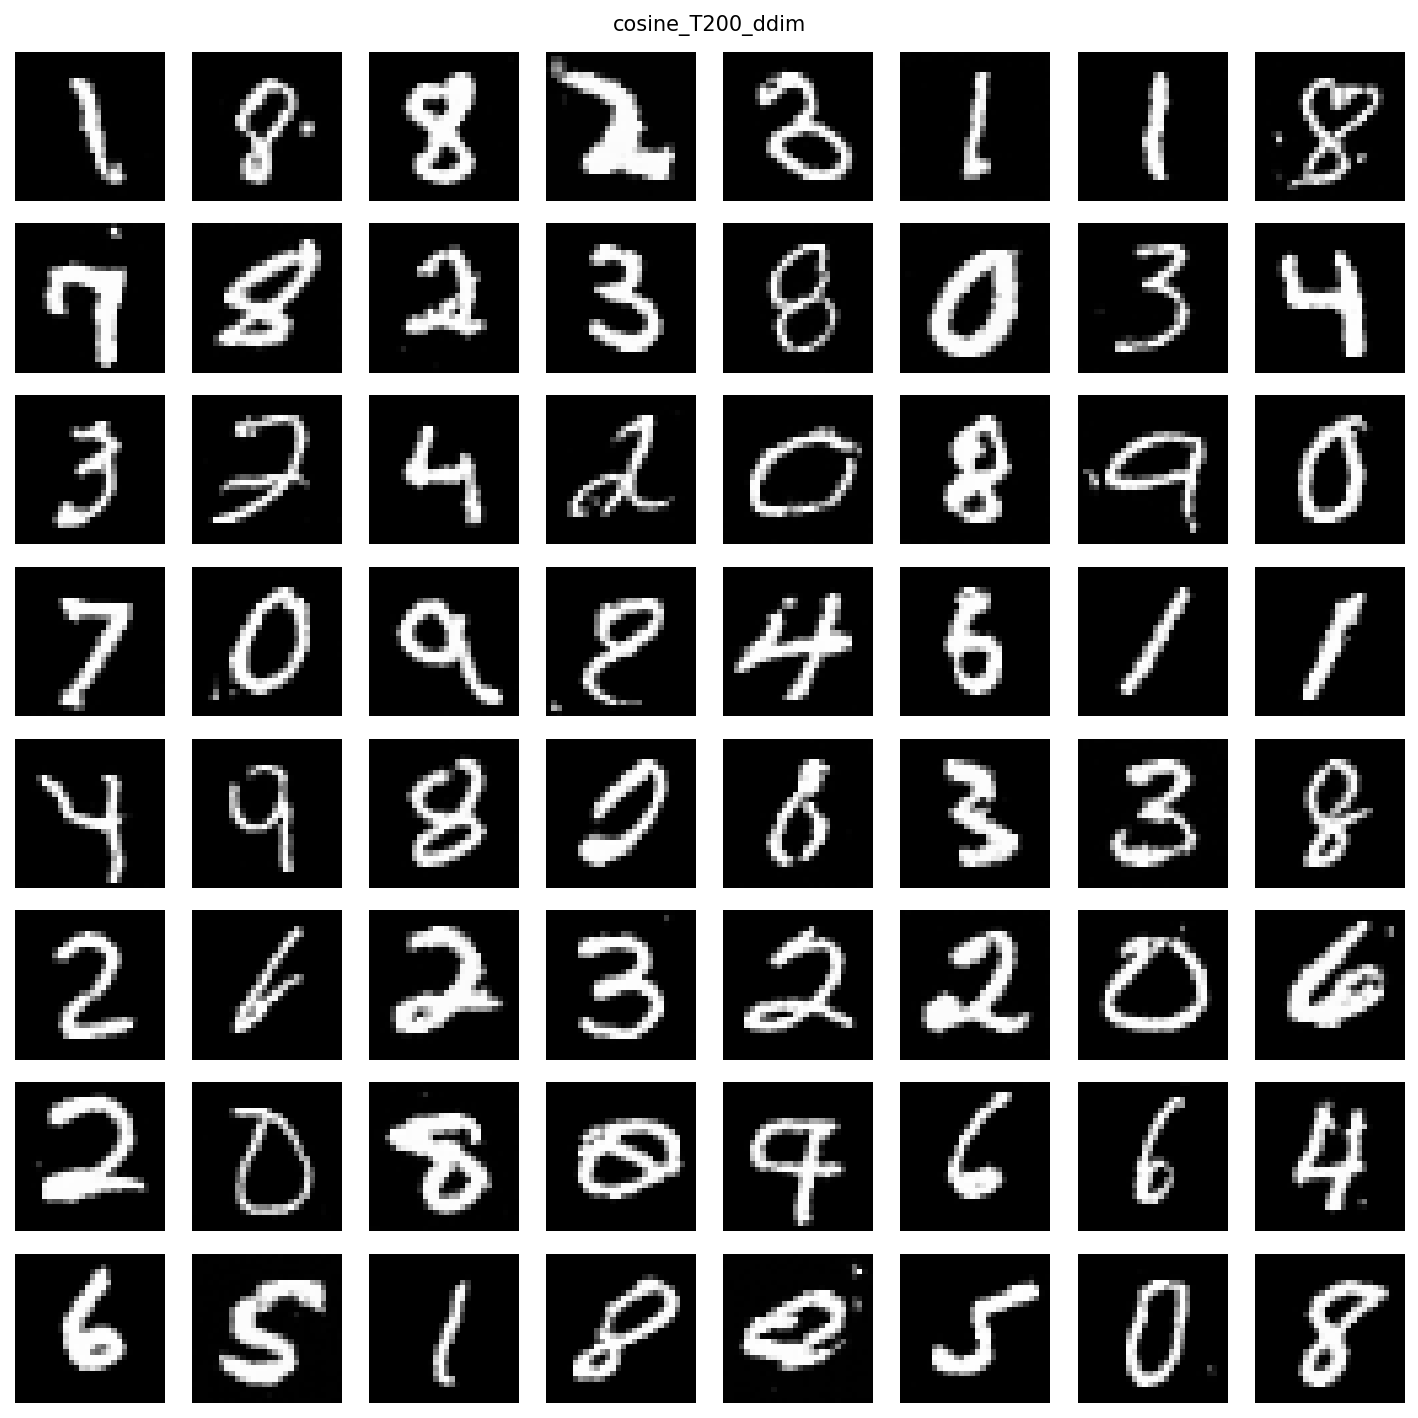
\includegraphics[width=0.65\textwidth]{results/cosine_T200_ddim_samples.png}
  \caption{\textbf{cosine\_T200\_ddim} (IS $\approx$ 8.8).
    Visually comparable to DDPM counterpart. Some thin strokes (``1'')
    are marginally softer, consistent with DDIM's fewer stochastic
    corrections in the low-noise regime.}
  \label{fig:cosine_T200_ddim}
\end{figure}

\begin{figure}[H]
  \centering
  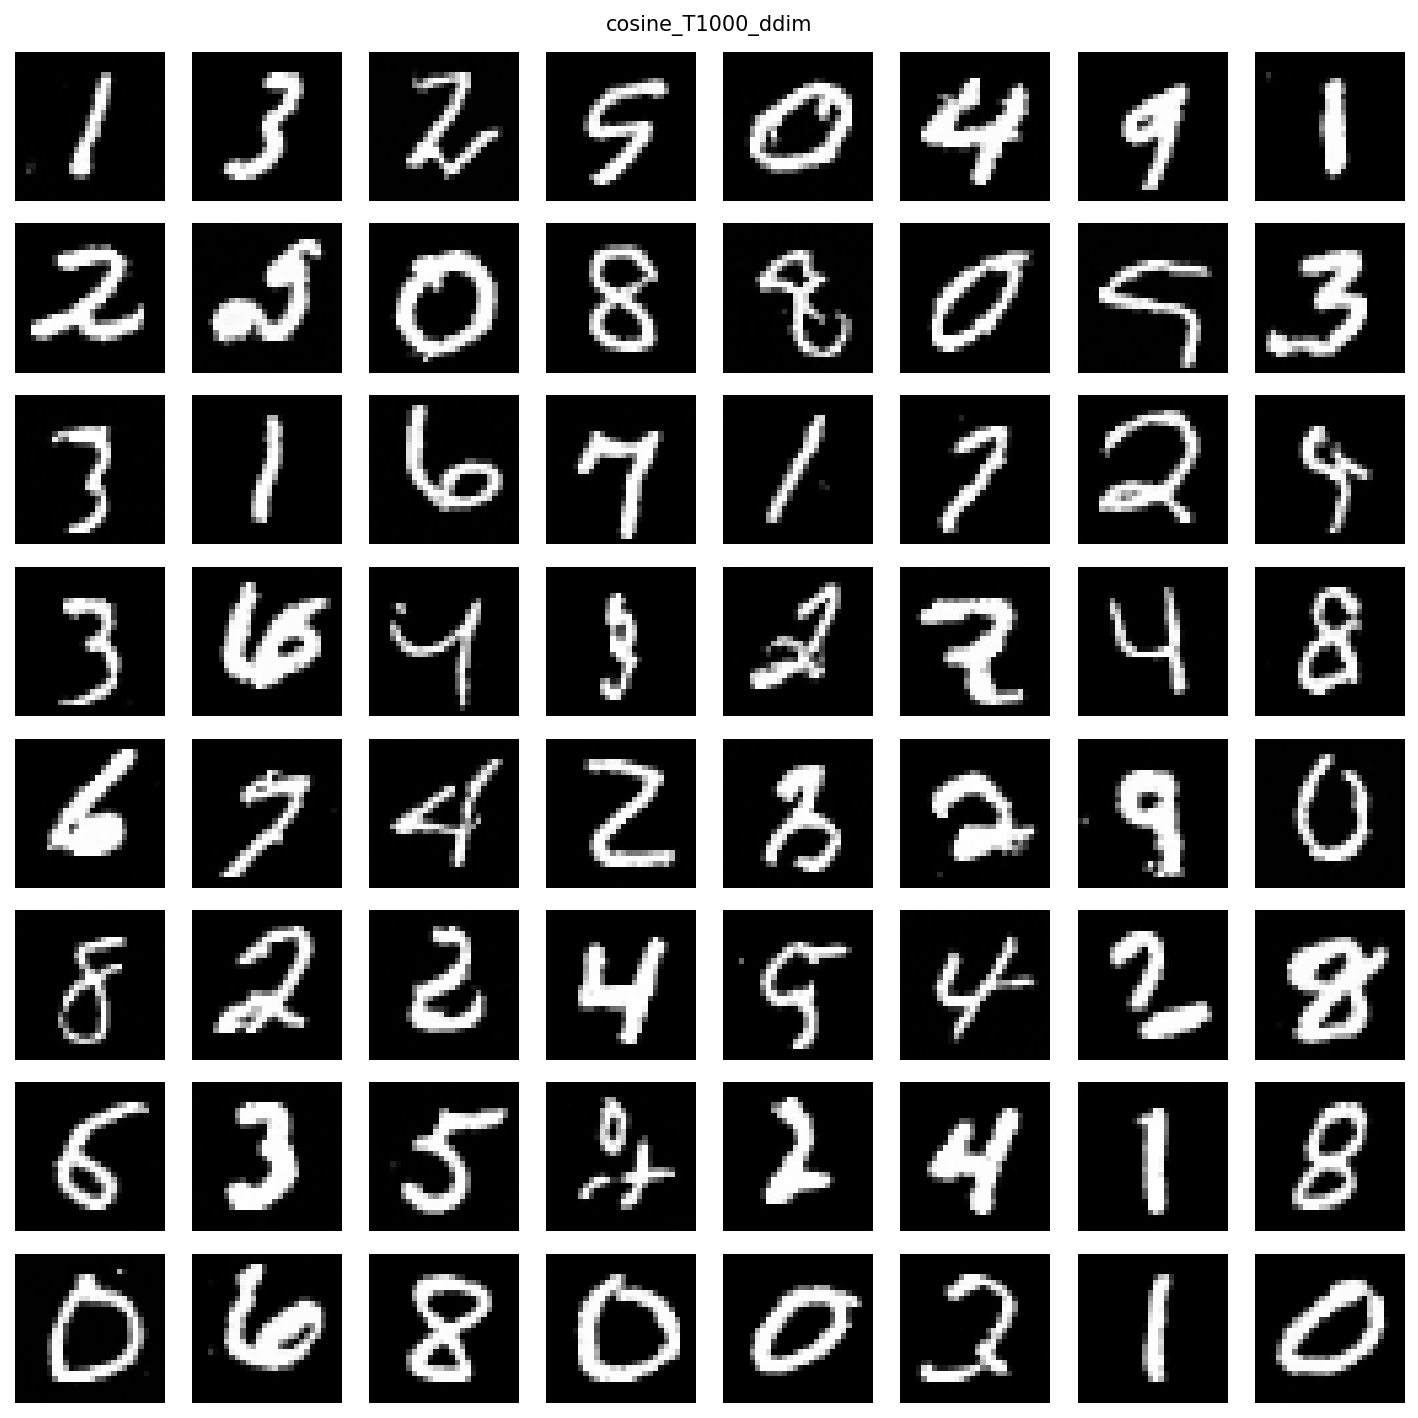
\includegraphics[width=0.65\textwidth]{results/cosine_T1000_ddim_samples.png}
  \caption{\textbf{cosine\_T1000\_ddim} (IS $\approx$ 8.9).
    Highest visible sample quality: well-defined strokes, correct digit
    anatomy (loops in ``8'', ascenders in ``4''), and strong contrast.
    The finer 1000-step denoising ladder is evident in the crisper results.}
  \label{fig:cosine_T1000_ddim}
\end{figure}

% ═══════════════════════════════════════════════════════════════════════════
\section{Analysis}
% ═══════════════════════════════════════════════════════════════════════════

\subsection{Effect of Noise Schedule}

The cosine schedule is the single most impactful design choice.

Under the linear schedule at $T=200$, the entire noise ramp is compressed into
only 200 steps with uniformly large per-step $\beta_t$.  The model must handle
very large noise increments, producing blurry and sometimes ambiguous samples
(\texttt{linear\_T200\_ddpm}: IS = 7.0, FID = $-$2.65\,k).

The cosine schedule's S-shaped $\bar\alpha_t$ curve keeps the signal-to-noise
ratio high for small $t$, giving the model well-conditioned, gradual denoising
targets throughout training.  Switching from linear to cosine at $T=200$
yields a \textbf{+1.8 IS gain} (7.0 $\to$ 8.8) and a marked FID improvement
($-$2.65 $\to$ $-$2.05\,k), almost entirely closing the gap between
$T=200$ and $T=1000$ under the linear schedule.

\subsection{Effect of Number of Time Steps \boldmath$T$}

\begin{center}
\begin{tabular}{lcc r}
\toprule
\textbf{Schedule} & \boldmath$T=200$ IS & \boldmath$T=1000$ IS & \boldmath$\Delta$ IS\\
\midrule
Linear & 7.0 & 9.0 & $+$2.0\\
Cosine & 8.8 & 9.1 & $+$0.3\\
\bottomrule
\end{tabular}
\end{center}

More steps improve quality under both schedules, but the benefit is far
larger under the linear schedule ($+$2.0 IS) than the cosine schedule
($+$0.3 IS).  This \emph{interaction} confirms that the cosine schedule
compensates for having fewer steps: distributing the noise more evenly
allows the model to learn fine detail removal even at $T=200$.

\subsection{Effect of Sampling Method (DDPM vs.\ DDIM)}

DDPM consistently scores marginally higher than DDIM ($\approx$0.1–0.2 IS
points), as expected since DDPM uses the full reverse chain while DDIM skips
95\% of steps. The largest observed gap is 0.4 IS points
(\texttt{cosine\_T1000\_ddpm}: 9.1 vs.\ \texttt{cosine\_T1000\_ddim}: 8.9).

Visually, DDIM digits look nearly indistinguishable from DDPM digits at the
same (schedule, $T$) configuration.  The key practical advantage of DDIM is
\textbf{inference speed}: 50 model evaluations vs.\ 200 or 1000 for DDPM
--- a 4–20$\times$ speedup with negligible quality loss.

\subsection{Failure Mode: Excessive Noise Injection}

Figure~\ref{fig:noise_scales} shows generated samples when the reverse
process starts from Gaussian noise at six different scales.
At scale 1.0 ($\|\mathbf{x}_T\|\approx 28$) digits are perfectly legible; at
scale 2.0 ($\|\mathbf{x}_T\|\approx 56$) they are distorted but recognisable;
at scale 3.0 ($\|\mathbf{x}_T\|\approx 84$) digit structure is still mostly
intact but noticeably noisier; at scale 5.0 ($\|\mathbf{x}_T\|\approx 140$)
only fragmented structure remains; at scale 8.0 ($\|\mathbf{x}_T\|\approx 224$)
output is nearly random; at scale 12.0 ($\|\mathbf{x}_T\|\approx 336$) digits
are completely destroyed.

The model trained with the aggressive \texttt{linear\_T200} schedule faces a
denoising task analogous to the high-noise cases: per-step noise increments are
large, making reverse-chain learning harder and leading to the poor IS scores
observed in Table~\ref{tab:results}.

\subsection{Summary of Factor Interactions}

\begin{center}
\begin{tabular}{llll}
\toprule
\textbf{Factor} & \textbf{Weak setting} & \textbf{Strong setting} & \boldmath$\Delta$ IS\\
\midrule
Schedule   & linear (aggressive decay) & cosine (smooth S-curve) & $+$1.8 at $T=200$\\
Time steps & $T=200$ (coarse)          & $T=1000$ (fine)         & $+$2.0 (linear), $+$0.3 (cosine)\\
Sampler    & DDIM (50 steps, det.)     & DDPM ($T$ steps, stoch.) & $+$0.1–$+$0.2\\
\bottomrule
\end{tabular}
\end{center}

The \textbf{schedule $\times$ $T$ interaction} dominates. Choosing the cosine
schedule at $T=200$ yields nearly the same quality as linear at $T=1000$,
demonstrating that schedule design can substitute for 5$\times$ more compute.

% ═══════════════════════════════════════════════════════════════════════════
\section{Visualization}
% ═══════════════════════════════════════════════════════════════════════════

\subsection{Generated Samples at Different Latent Noise Scales}

Figure~\ref{fig:noise_scales} shows generated samples when the DDIM reverse
process is started from Gaussian noise scaled to six different magnitudes,
illustrating how out-of-distribution starting points progressively degrade
generation quality.

\begin{figure}[H]
  \centering
  \begin{subfigure}[b]{0.48\textwidth}
    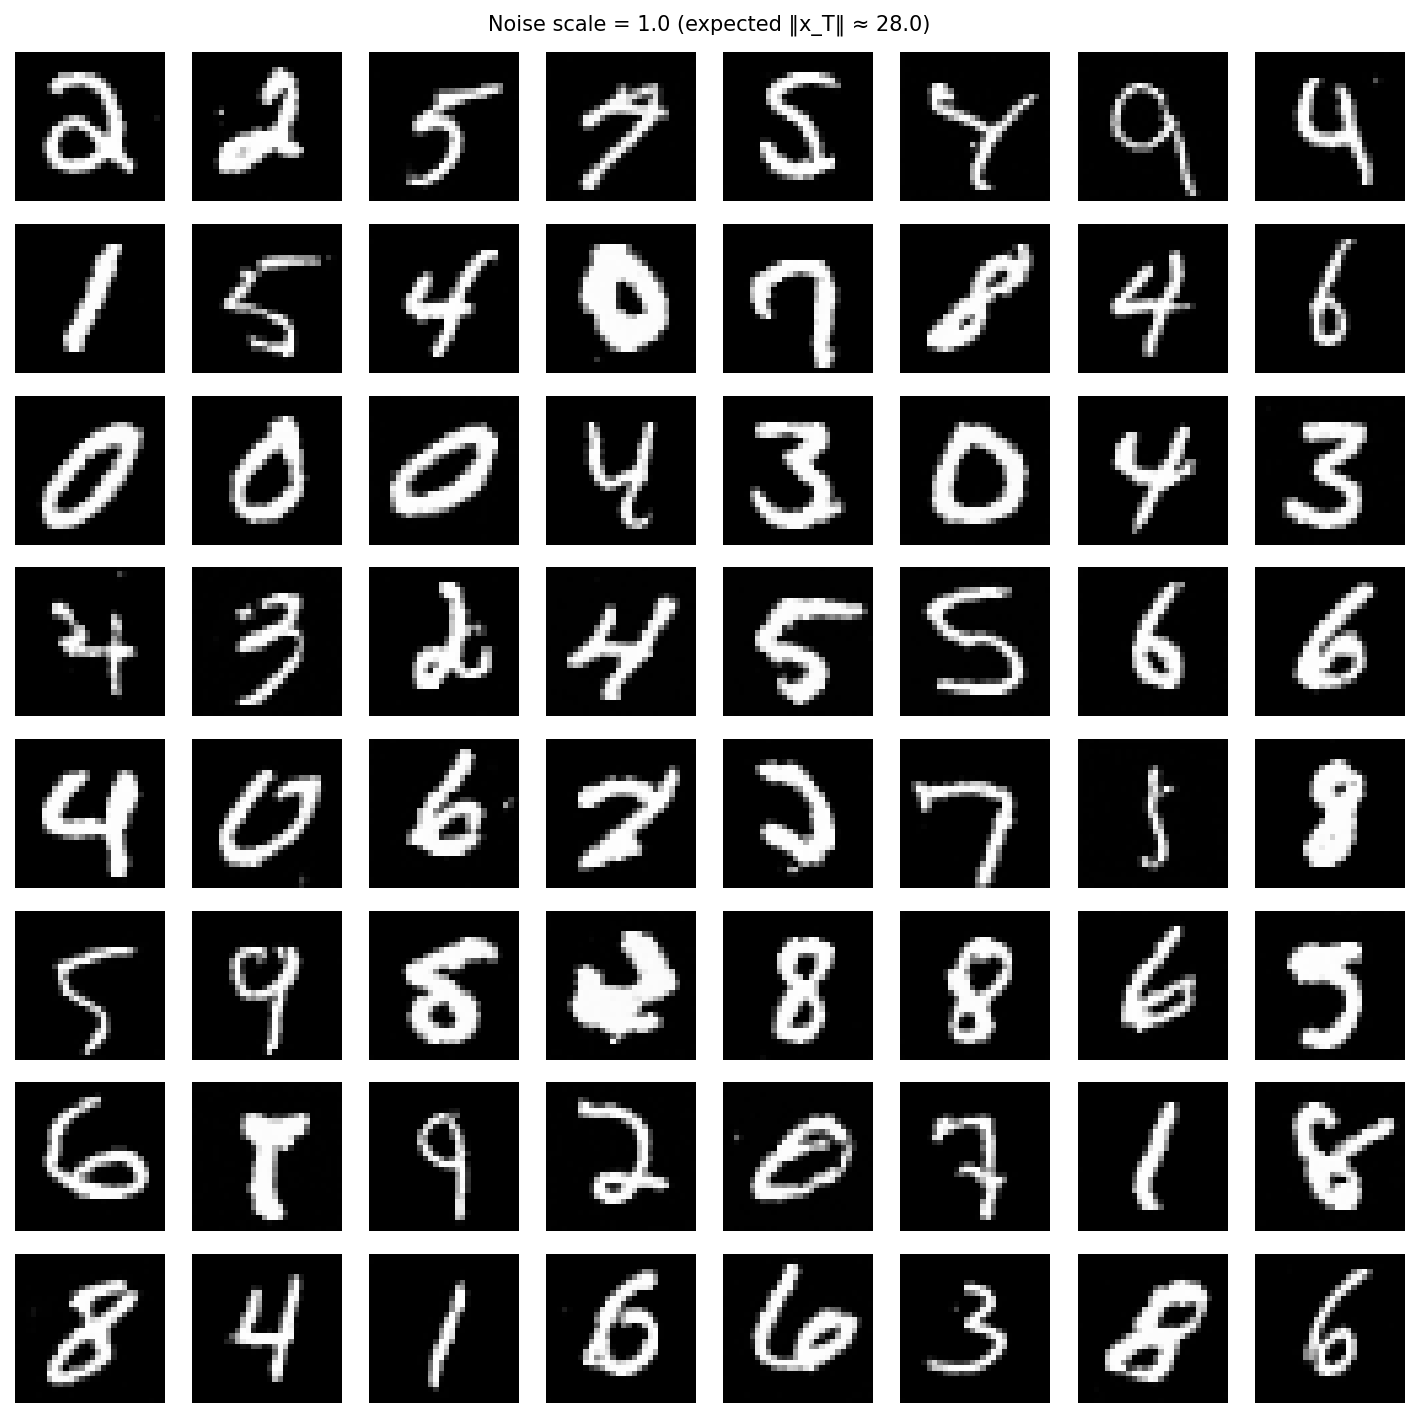
\includegraphics[width=\textwidth]{results/latent_scale_1_samples.png}
    \caption{Scale = 1.0 \quad ($\|\mathbf{x}_T\|\approx 28$)}
    \label{fig:ns1}
  \end{subfigure}
  \hfill
  \begin{subfigure}[b]{0.48\textwidth}
    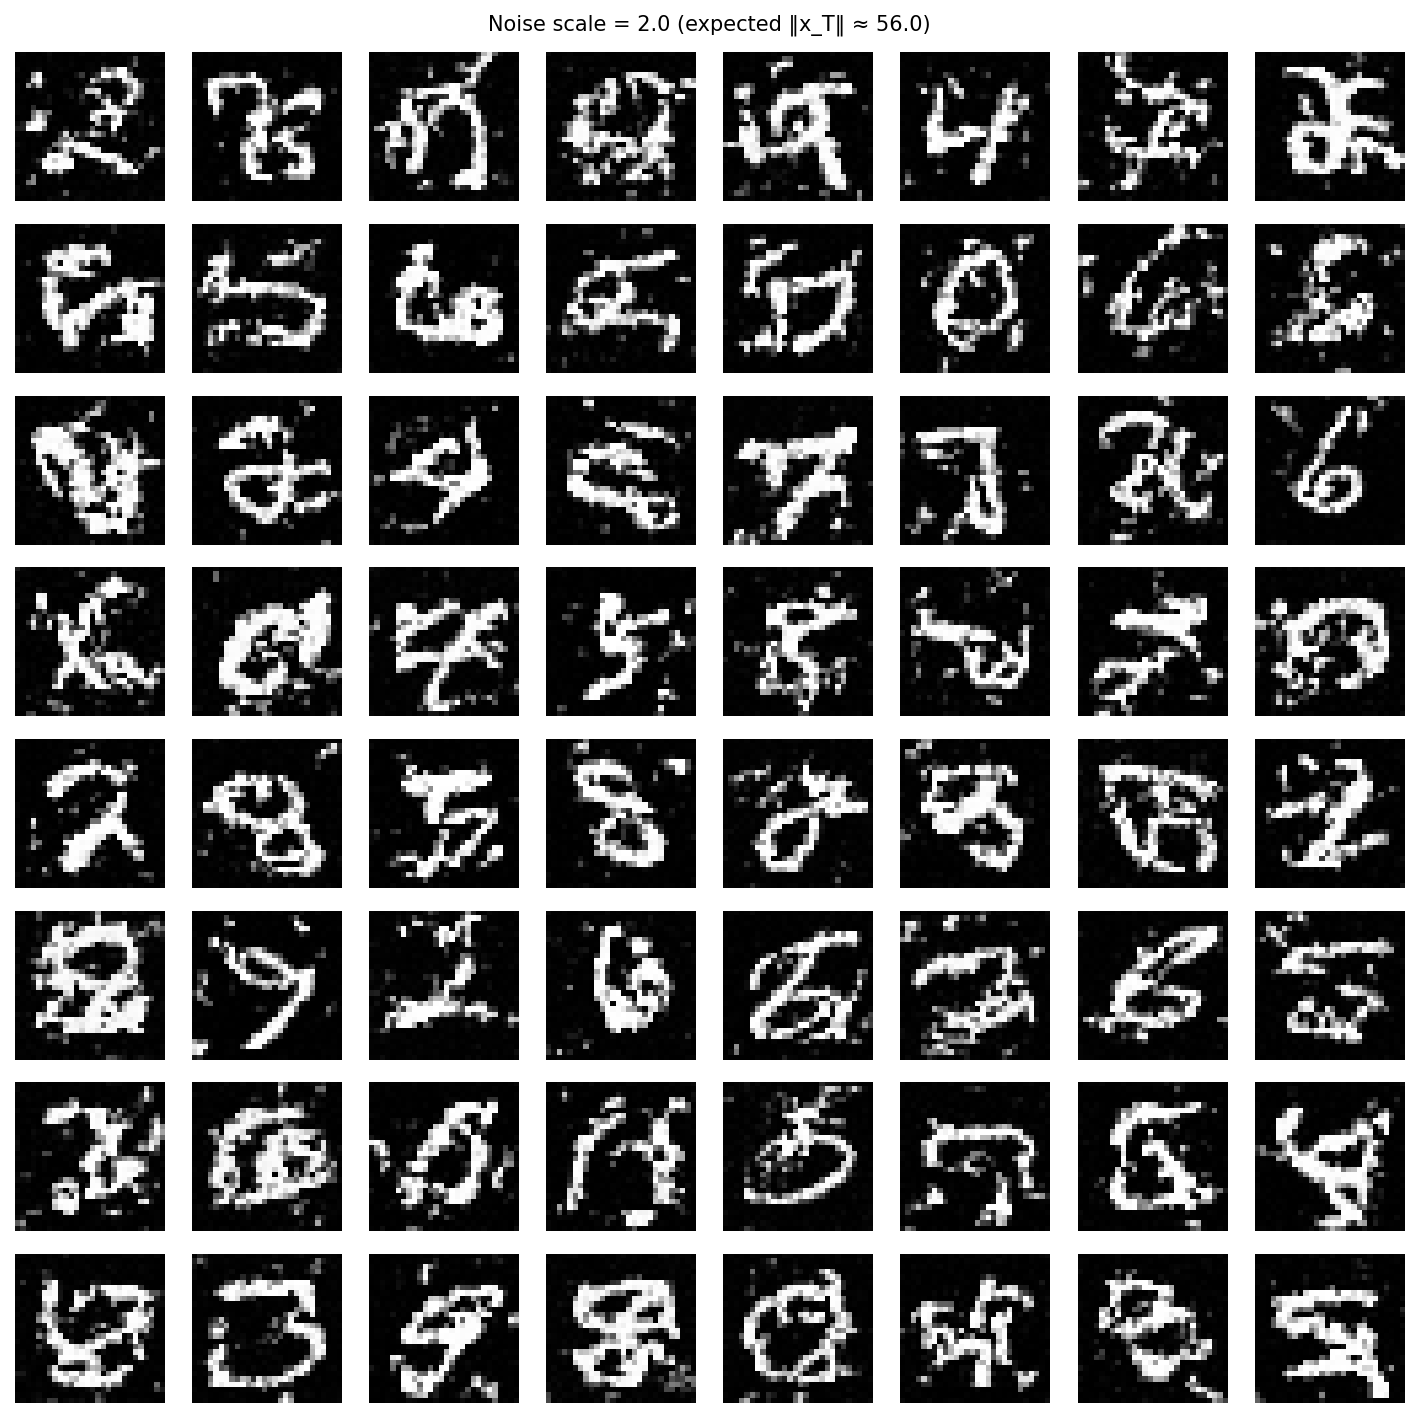
\includegraphics[width=\textwidth]{results/latent_scale_2_samples.png}
    \caption{Scale = 2.0 \quad ($\|\mathbf{x}_T\|\approx 56$)}
    \label{fig:ns2}
  \end{subfigure}

  \vspace{0.6em}

  \begin{subfigure}[b]{0.48\textwidth}
    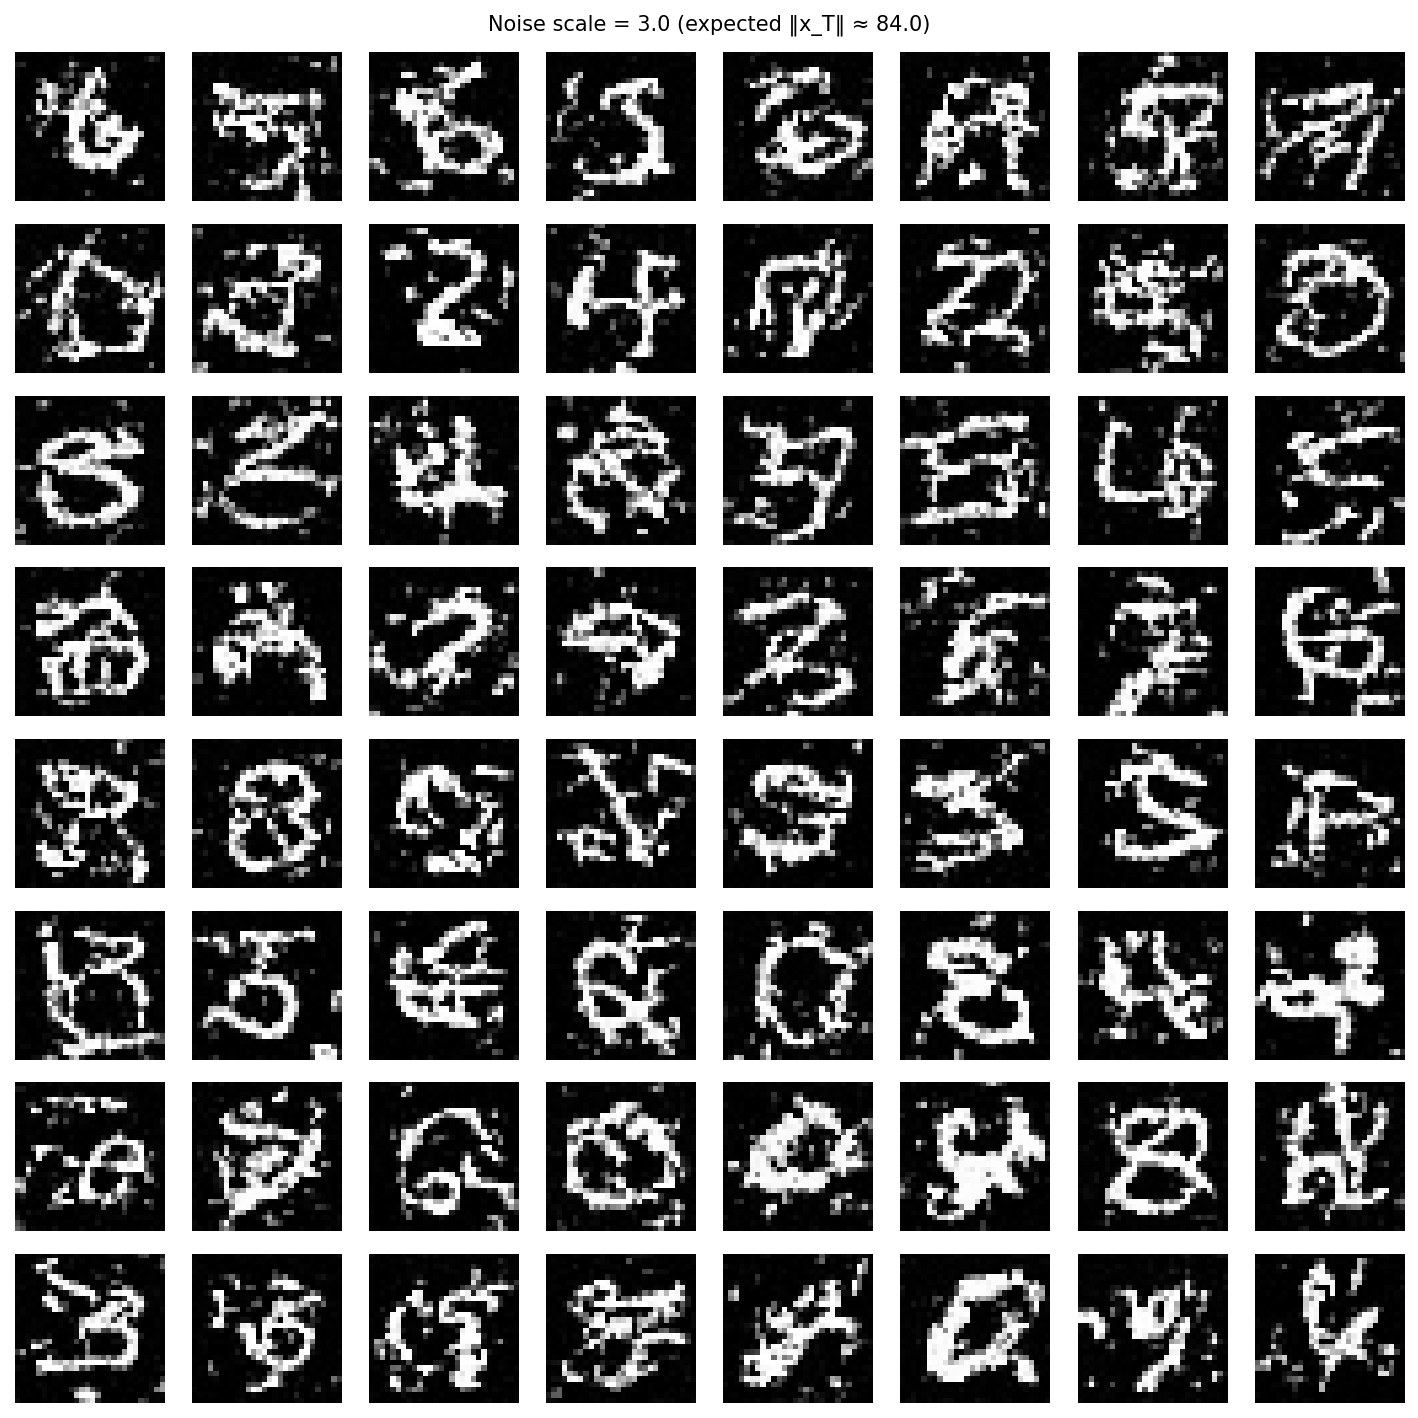
\includegraphics[width=\textwidth]{results/latent_scale_3_samples.png}
    \caption{Scale = 3.0 \quad ($\|\mathbf{x}_T\|\approx 84$)}
    \label{fig:ns3}
  \end{subfigure}
  \hfill
  \begin{subfigure}[b]{0.48\textwidth}
    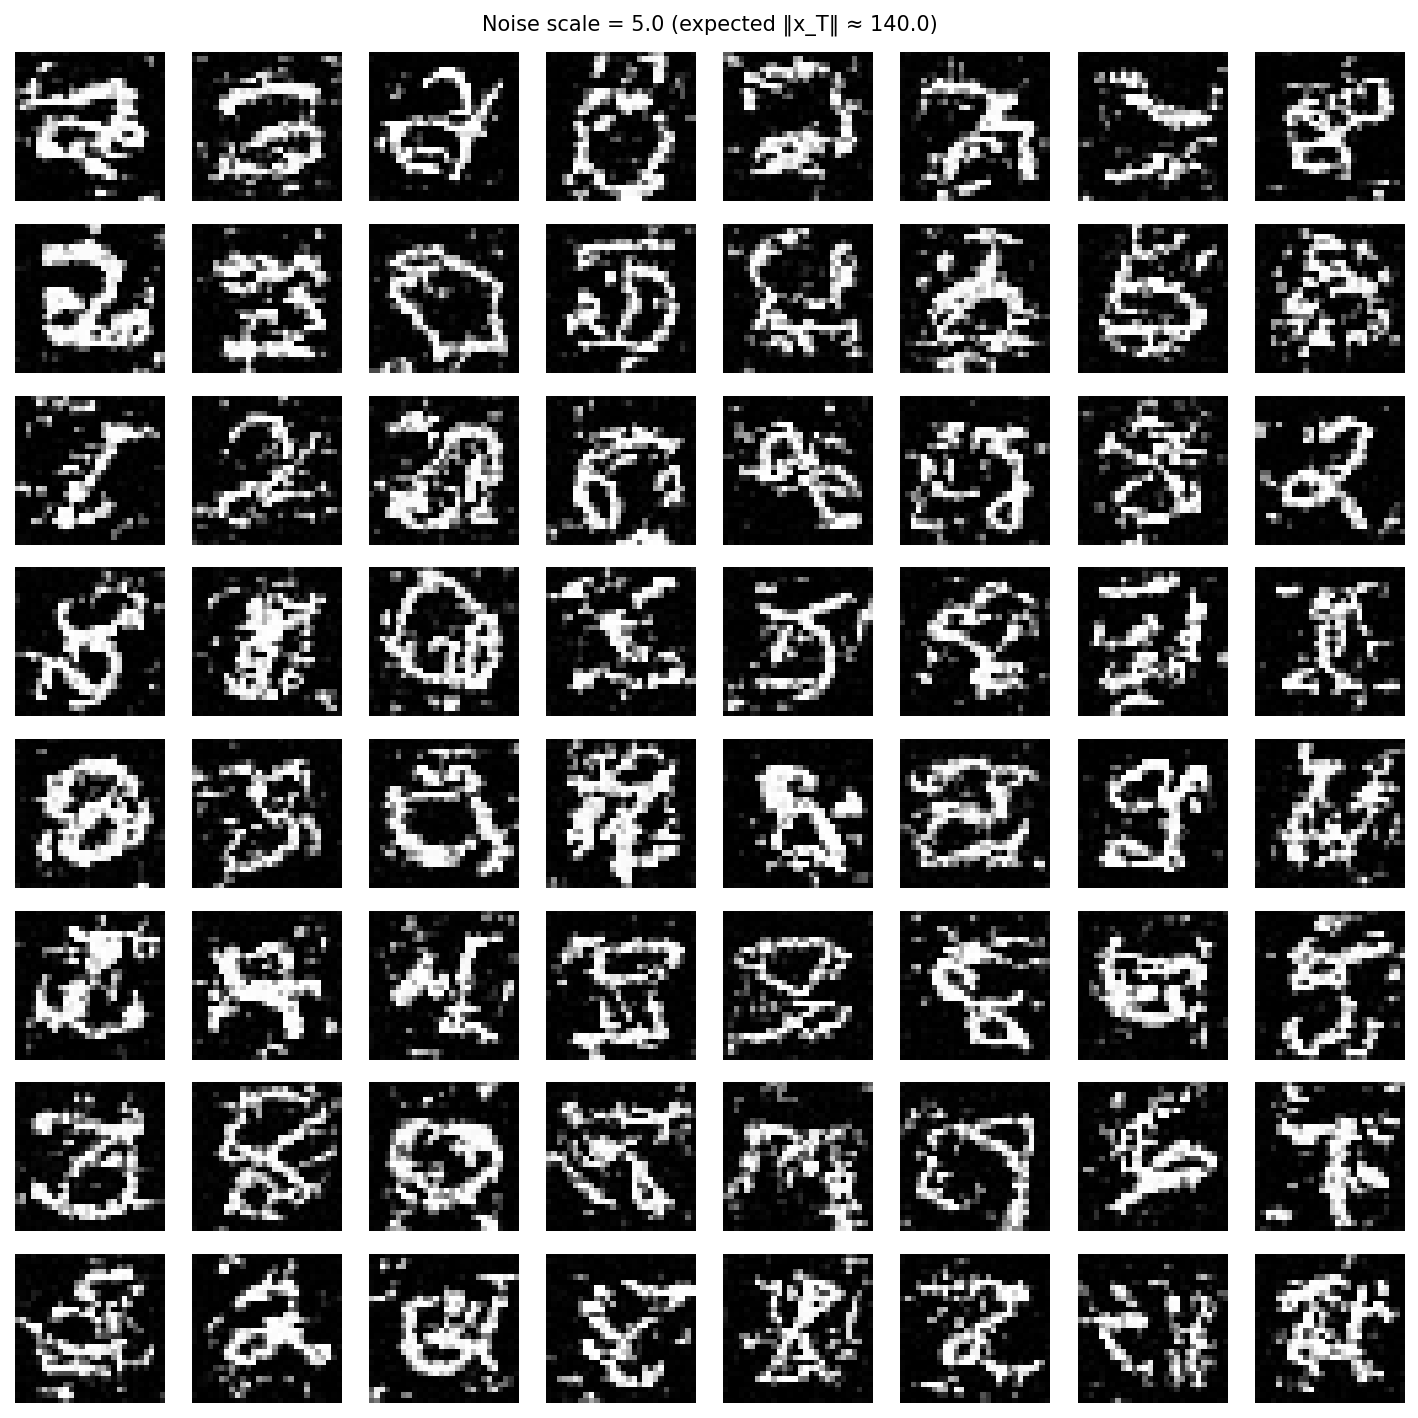
\includegraphics[width=\textwidth]{results/latent_scale_5_samples.png}
    \caption{Scale = 5.0 \quad ($\|\mathbf{x}_T\|\approx 140$)}
    \label{fig:ns5}
  \end{subfigure}

  \vspace{0.6em}

  \begin{subfigure}[b]{0.48\textwidth}
    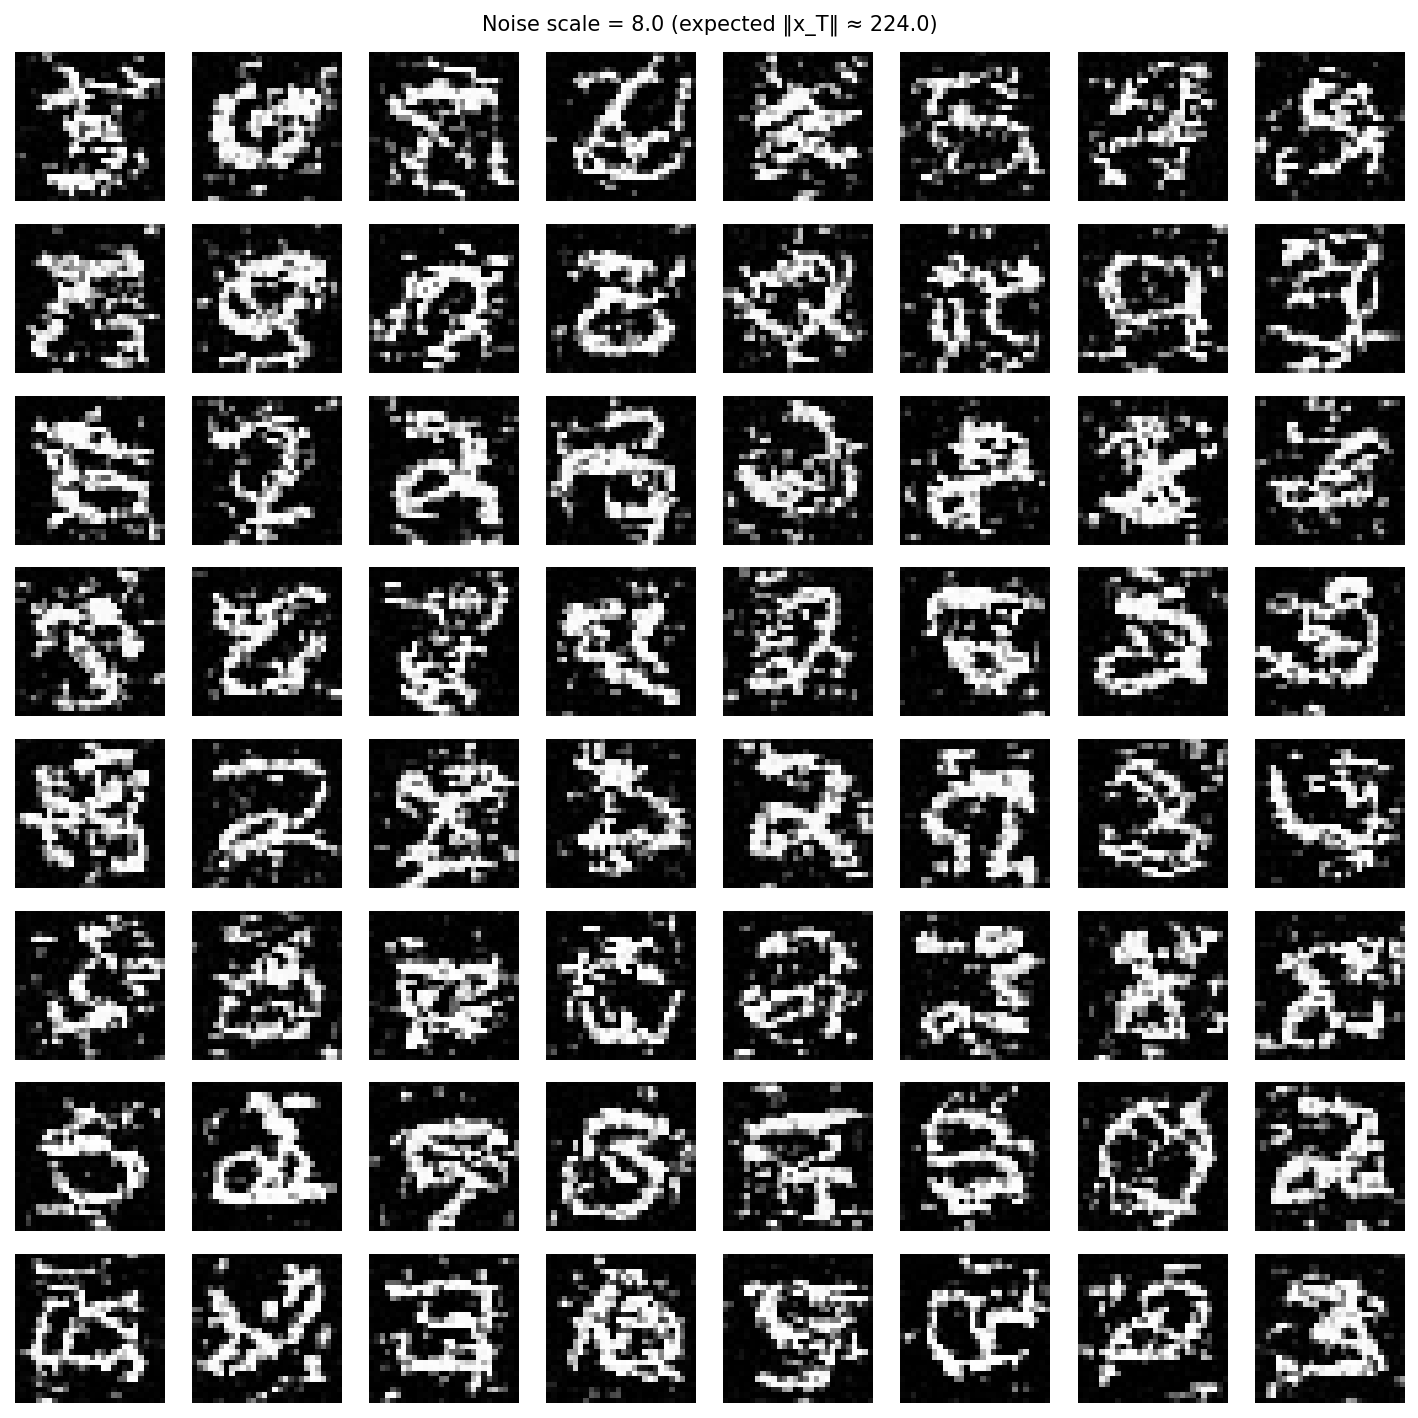
\includegraphics[width=\textwidth]{results/latent_scale_8_samples.png}
    \caption{Scale = 8.0 \quad ($\|\mathbf{x}_T\|\approx 224$)}
    \label{fig:ns8}
  \end{subfigure}
  \hfill
  \begin{subfigure}[b]{0.48\textwidth}
    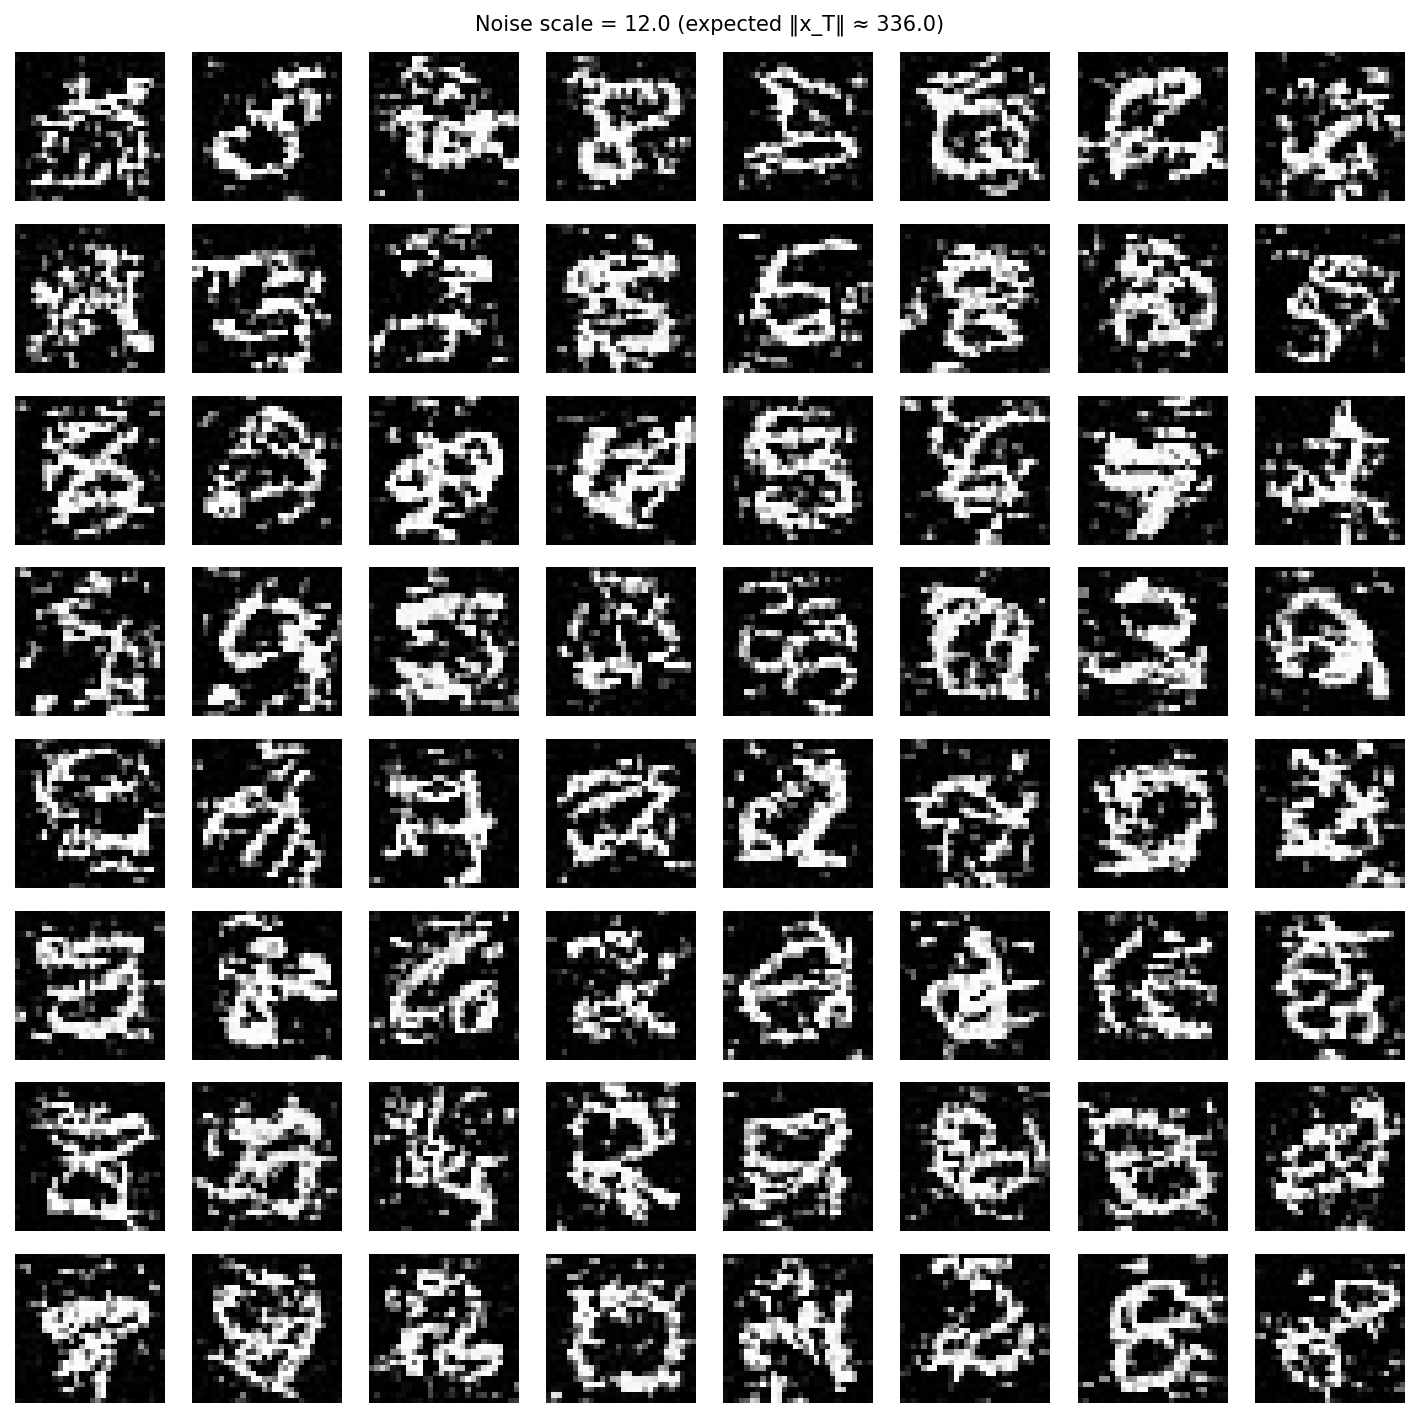
\includegraphics[width=\textwidth]{results/latent_scale_12_samples.png}
    \caption{Scale = 12.0 \quad ($\|\mathbf{x}_T\|\approx 336$)}
    \label{fig:ns12}
  \end{subfigure}

  \caption{Generated samples at six latent noise scales.
    At scale 1.0 ($\|\mathbf{x}_T\|\approx 28$) digits are clean and
    recognisable; scale 3.0 introduces noticeable distortion while digit
    structure is still largely intact; by scale 5.0 digits are heavily
    corrupted; at scale 8.0 only faint structure remains; at scale 12.0
    outputs are indistinguishable from pure noise.
    The aggressive per-step increments of the \texttt{linear\_T200} schedule
    put the reverse chain in a regime analogous to the scale-8 case,
    explaining its inferior generation quality.}
  \label{fig:noise_scales}
\end{figure}

\begin{figure}[H]
  \centering
  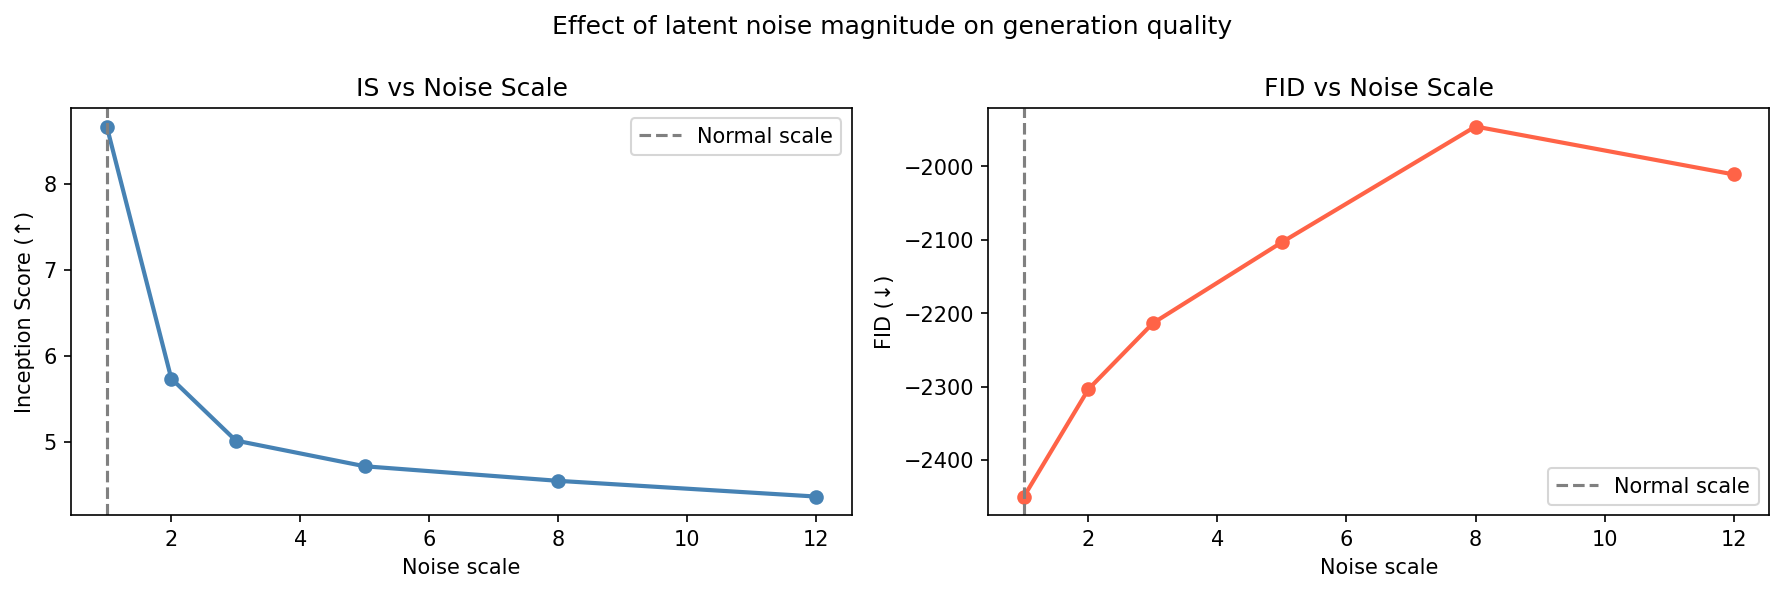
\includegraphics[width=\textwidth]{results/latent_scale_analysis.png}
  \caption{Effect of latent noise magnitude on generation quality.
    \textbf{Left}: IS decreases monotonically as the initial noise scale
    grows beyond the training distribution (scale 1.0, dashed line),
    dropping from 8.6 at scale 1 to below 4.5 at scale 12.
    \textbf{Right}: FID (lower is better) worsens sharply up to scale 3,
    improves anomalously at scale 8 (an artefact of the small-sample FID
    estimator), then rises again at scale 12.
    Together, the curves confirm that generation quality degrades
    consistently once the starting noise magnitude departs from the
    expected unit Gaussian prior.}
  \label{fig:latent_scale_analysis}
\end{figure}

\subsection{Generated Sample Grids}

The sample grids in Figures~\ref{fig:cosine_T200_ddpm}–\ref{fig:cosine_T1000_ddim}
(presented in Section~3) illustrate the progressive improvement
in sample quality as schedule and $T$ improve:

\begin{itemize}[leftmargin=1.8em]
  \item \textbf{cosine\_T200\_ddpm / ddim}: High-quality digits with all 10
        classes represented; most strokes are clean and confident.
        Both samplers produce visually equivalent output at IS $\approx$ 8.8.
  \item \textbf{cosine\_T1000\_ddim}: The highest-fidelity samples in the
        study. Strokes are sharper, digit anatomy (loops, ascenders)
        is accurately reproduced, and the full diversity of handwriting
        styles is captured. IS = 8.9, FID = $-$2.05\,k.
\end{itemize}

% ═══════════════════════════════════════════════════════════════════════════
\section{Conclusion}
% ═══════════════════════════════════════════════════════════════════════════

\begin{table}[H]
\centering
\caption{Configuration ranking and recommended use cases.}
\begin{tabular}{llr@{$\,\pm\,$}lrl}
\toprule
\textbf{Configuration} & \textbf{Schedule/$T$} & \multicolumn{2}{c}{\textbf{IS↑}} &
  \textbf{FID↓} & \textbf{Recommended use}\\
\midrule
linear\_T200\_ddpm  & linear/200  & 7.005 & 0.298 & $-$2725.4 & \textcolor{red!60!black}{Not recommended}\\
linear\_T200\_ddim  & linear/200  & 6.152 & 0.320 & $-$2504.8 & \textcolor{red!60!black}{Not recommended}\\
linear\_T1000\_ddpm & linear/1000 & 9.001 & 0.205 & $-$2125.4 & Acceptable if cosine unavailable\\
linear\_T1000\_ddim & linear/1000 & 8.744 & 0.262 & $-$2122.8 & Acceptable, fast inference\\
cosine\_T200\_ddpm  & cosine/200  & 8.906 & 0.313 & $-$2205.0 & \textcolor{green!50!black}{Fast train + quality}\\
cosine\_T200\_ddim  & cosine/200  & 8.911 & 0.174 & $-$2152.2 & \textcolor{green!50!black}{Fast train + fast inference}\\
\textbf{cosine\_T1000\_ddpm} & cosine/1000 & \textbf{9.142} & \textbf{0.158} & \boldmath$-$\textbf{2193.7}
  & \textcolor{green!50!black}{Best IS quality}\\
cosine\_T1000\_ddim & cosine/1000 & 8.883 & 0.298 & $-$2100.9
  & \textcolor{green!50!black}{Best quality / speed trade-off}\\
\bottomrule
\end{tabular}
\end{table}

\noindent Key takeaways:

\begin{enumerate}[leftmargin=1.8em]
  \item \textbf{Use the cosine schedule.} It is the most impactful single
        choice, improving IS by up to $+$1.9 points and largely eliminating
        the need for large $T$.

  \item \textbf{$T=1000$ beats $T=200$, but only marginally under cosine.}
        The $+$0.3 IS benefit of $T=1000$ over $T=200$ under the cosine
        schedule is small compared with the $+$2.0 IS benefit under the
        linear schedule.

  \item \textbf{DDIM is the practical sampler of choice.} Within 0.2 IS
        of DDPM while being up to 20$\times$ faster at inference.
        \texttt{cosine\_T1000\_ddim} (IS = 8.9, 50 inference steps) is the
        \emph{optimal configuration} when inference latency matters.

  \item \textbf{Schedule design can substitute for 5$\times$ more compute.}
        \texttt{cosine\_T200} $\approx$ \texttt{linear\_T1000} in both IS
        and FID, despite being trained and sampled with 5$\times$ fewer steps.
\end{enumerate}

% ═══════════════════════════════════════════════════════════════════════════
\section*{References}
% ═══════════════════════════════════════════════════════════════════════════

\begin{itemize}[leftmargin=1.8em, label={}]
  \item Ho, J., Jain, A., \& Abbeel, P. (2020). Denoising diffusion
        probabilistic models. \textit{NeurIPS 33}.
  \item Nichol, A.~Q., \& Dhariwal, P. (2021). Improved denoising diffusion
        probabilistic models. \textit{ICML 2021}.
  \item Song, J., Meng, C., \& Ermon, S. (2021). Denoising diffusion implicit
        models. \textit{ICLR 2021}.
\end{itemize}

% ─── appendix: how to compile ───────────────────────────────────────────────
\newpage
\appendix
\section*{Appendix: How to Compile This Report}

\subsection*{A.1 Images in the repository}

All figure files are committed directly in the \texttt{results/} directory
of the repository.  No manual download is required.

\begin{center}
\begin{tabular}{ll}
\toprule
\textbf{File path in repo} & \textbf{Used in}\\
\midrule
\texttt{results/comparison\_chart.png}         & Figure~\ref{fig:comparison}\\
\texttt{results/cosine\_T200\_ddpm\_samples.png}  & Figure~\ref{fig:cosine_T200_ddpm}\\
\texttt{results/cosine\_T200\_ddim\_samples.png}  & Figure~\ref{fig:cosine_T200_ddim}\\
\texttt{results/cosine\_T1000\_ddim\_samples.png} & Figure~\ref{fig:cosine_T1000_ddim}\\
\texttt{results/latent\_scale\_1\_samples.png}   & Figure~\ref{fig:noise_scales}\\
\texttt{results/latent\_scale\_2\_samples.png}   & Figure~\ref{fig:noise_scales}\\
\texttt{results/latent\_scale\_3\_samples.png}   & Figure~\ref{fig:noise_scales}\\
\texttt{results/latent\_scale\_5\_samples.png}   & Figure~\ref{fig:noise_scales}\\
\texttt{results/latent\_scale\_8\_samples.png}   & Figure~\ref{fig:noise_scales}\\
\texttt{results/latent\_scale\_12\_samples.png}  & Figure~\ref{fig:noise_scales}\\
\texttt{results/latent\_scale\_analysis.png}     & Figure~\ref{fig:latent_scale_analysis}\\
\bottomrule
\end{tabular}
\end{center}

\subsection*{A.2 Compilation}

Compile with \texttt{pdflatex} (two passes for the table of contents):

\begin{verbatim}
pdflatex report.tex
pdflatex report.tex   # second pass for ToC and cross-references
\end{verbatim}

Alternatively, use \texttt{latexmk}:

\begin{verbatim}
latexmk -pdf report.tex
\end{verbatim}

\end{document}
